\subsection{State Estimation}
\label{subsec:SE}

We evaluate \genco on State Estimation (SE), the task of recovering bus voltage magnitudes and phase angles from noisy, incomplete, and corrupted measurements. Classical state estimators formulate SE as a nonlinear inverse problem, most commonly solved using Weighted Least Squares (WLS), which relies on an accurate grid model and a sufficiently informative (i.e. locally observable) measurement set. In contrast, \genco learns a direct mapping from measurements to grid states by combining data-driven priors with physics-informed corrections, as described in \cref{sec:model}. % Rather than explicitly solving the inverse problem at inference time, it leverages the distribution of operating conditions observed during training together with physics-based corrective updates. 
We first evaluate its robustness to sparse, noisy, and outlier-corrupted measurements, as well as cases where WLS fails to converge, before studying its resilience to inaccuracies in the underlying grid model caused by admittance parameter errors.


\paragraph{Experimental setup.} GENCO models are trained on datasets generated via \datakit, comprising roughly 250{,}000 scenarios per grid, with varying N-k topology perturbations ($k=5$ for IEEE 14/30/57 and $k=10$ for IEEE 118) and admittance perturbations, on the standard IEEE 14, 30, 57, and 118-bus systems. In the absence of standardized datasets and procedures for generating synthetic SCADA measurements, we define our measurement-generation protocol and evaluation settings as follows. We generate SCADA measurements from the true bus voltage magnitudes $V$, bus power injections $P_{\text{inj}}, Q_{\text{inj}}$, and branch flows $P_{\text{flow}}, Q_{\text{flow}}$ by applying three different types of perturbations; first, we randomly mask a fraction $p_{\text{mask}}$ of the available measurements to emulate limited measurement coverage, with the resulting number of measurements expressed as a multiple of the number of buses $|\mathcal{N}|$; second, we apply multiplicative Gaussian noise ($\sigma_V = 0.01$~p.u., $\sigma_{P,Q} = 0.02$~p.u.) to all measurements, independently perturbing each measured voltage magnitude, active/reactive power injection, and active/reactive branch flow; third, we create outliers by adding a bias of three standard deviations to a fraction $p_{\text{outlier}}$ of measurements. We consider arbitrary measurement locations, but do not enforce sensor placement according to power-system observability rules. To mitigate this simplification, we use measurement densities above typical observability requirements (at least $5|\mathcal{N}|$ measurements, compared to the commonly used $4|\mathcal{N}|$ rule of thumb\footnote{\url{https://pandapower.readthedocs.io/en/latest/estimation.html}}, and $3.2 \text{ to } 4.6|\mathcal{N}|$ measurements used by Hydro-Québec~\cite{4596318}) and report results only on scenarios that remain observable under WLS. Voltage angles are never measured. To train GENCO models, we use $p_{\text{mask}} = 0.2$ and $p_{\text{outlier}} = 0.1$ and minimize the loss shown in \cref{eq:loss}, with $\mathcal{L}_{\text{supervised}}$ being the mean $\ell_1$ norm between true and predicted bus and edge variables.


% 345 kV maps closest to HQ's 3XX (315 kV) tier — highest-redundancy tier below the 735 kV backbone, m/n ≈ 3.7–4.6.
% 138 kV maps closest to HQ's 1XX (120–161 kV) tier — the largest single tier by measurement count (1413), with moderate redundancy, m/n ≈ 3.2–4.0.
% https://ieeexplore.ieee.org/document/4596318

\paragraph{Baseline and evaluation.} We compare \genco against a Weighted Least Squares (WLS) baseline solved with the Gauss--Newton (GN) algorithm and outlier rejection, using the pandapower implementation~\cite{pandapower}. WLS receives the standard deviations of the measurements, giving it an advantage over \genco, which must implicitly infer measurement uncertainty from the training distribution. We evaluate each scenario using the bus-averaged mean absolute error. In rare under-determined scenarios, WLS can converge to a solution substantially different from the reference state while remaining consistent with the measurements, producing large errors that disproportionately affect the mean. We therefore use the median across scenarios of the bus-averaged mean absolute error as our primary metric, reducing the influence of such cases without requiring an arbitrary threshold to identify and exclude them. The baseline is evaluated only when the measurement-function Jacobian is full rank; comparisons are thus reported on that subset. Results for cases where the baseline does not converge are shown in \cref{fig:non-observable} in \cref{app:se}. \


\paragraph{Robustness to sparse, noisy, and outlier measurements.}
We first evaluate \genco against WLS with varying numbers of measurements and outlier rates in \cref{fig:base-case}. One GENCO model is trained for each grid and evaluated across all measurement densities and outlier levels. Overall, \genco reconstructs states more accurately than WLS on the small grids---its median voltage magnitude error is up to an order of magnitude lower on the IEEE 14- and 30-bus cases---with a degradation on the larger grids. %More importantly, while WLS fails to converge on 1--6\% of the cases, \genco always returns a solution.\\
\\



\begin{figure}
    \centering
    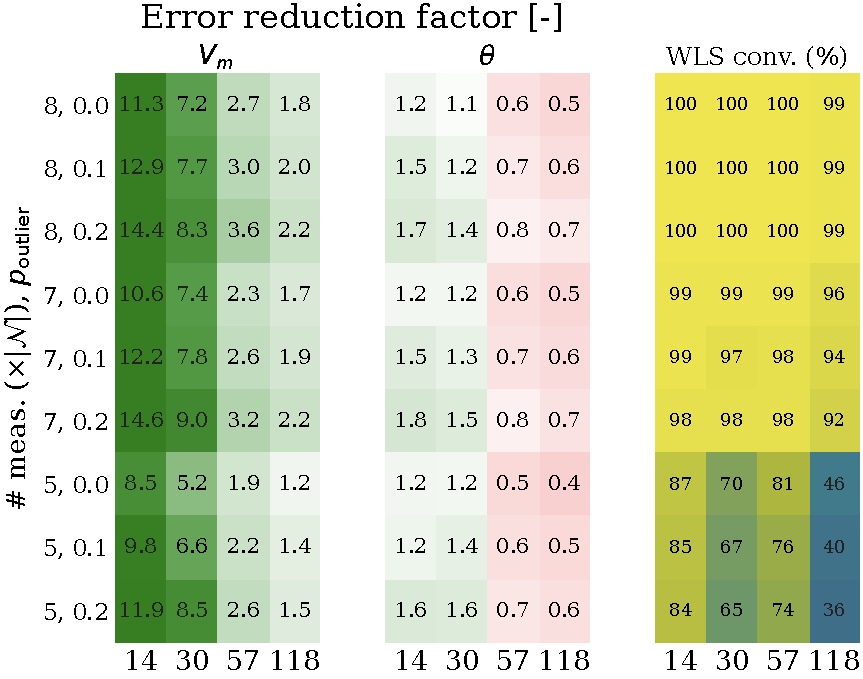
\includegraphics[width=\linewidth]{figures/se/base_case.pdf}
    \caption{State-estimation accuracy for varying numbers of noisy measurements and outlier probabilities. The first two panels show the error ratio of \genco relative to the WLS baseline (ratio of their median mean absolute errors) per variable: values above $1$ (green) indicate that \genco is more accurate, whereas values below $1$ (red) favor the baseline. The last column represents the percentage of scenarios in which the baseline converges; \genco always returns an estimate. Columns correspond to the IEEE 14-, 30-, 57-, and 118-bus grids.}
    \label{fig:base-case}
\end{figure}

As measurements become sparser and more corrupted, \genco remains robust, increasingly outperforming WLS on small grids and closing the gap with pandapower on larger grids. Note that the reported accuracy is computed only over scenarios where WLS converges, the number of which shrinks as measurements become sparser. \genco provides a complete estimator: unlike WLS, it returns an estimate even when the measurement configuration is insufficient for convergence. To assess the performance in cases where no WLS reference exists, \cref{fig:non-observable} reports the ratio between the errors of the non-converged and the converged subsets. Averaged across all sparsity levels, outlier rates, and grid-size settings, this ratio is $\approx 1.11$---a $\sim 10\%$ error increase on the cases where WLS yields no output at all. \genco thus degrades gracefully rather than failing abruptly, making it the more dependable estimator under marginal observability. Further improvements are required on larger grids, where \genco achieves the greatest gains in convergence robustness but falls short of WLS in accuracy.





\paragraph{Robustness to inaccurate grid parameters.}

While base grid parameters (e.g., admittance) are known to operators, they can drift throughout the day due to, e.g., temperature variations, which affect electrical resistance and the thermal expansion of transmission lines, resulting in line sag modulating the shunt capacitance. Consequently, the true grid parameters differ from the nominal parameters used by the state estimator. In \cref{fig:perturbation}, we evaluate \genco under grid parameter errors by perturbing the admittance with multiplicative factors sampled from a uniform distribution between $[1-\sigma_Y, 1+\sigma_Y]$. During training, measurements were consistent with the grid parameters, whereas during evaluation, the test set contains measurements that are generated using perturbed parameters, while the estimator receives the nominal admittance. Because \genco treats the grid physics as a soft prior rather than a hard constraint, it absorbs these discrepancies and keeps improving over the baseline as $\sigma_Y$ grows. In comparison, WLS enforces the now-incorrect model equations, causing the outlier-rejection procedure to incorrectly flag valid measurements and making non-convergence increasingly likely.\\


\begin{figure}
    \centering
    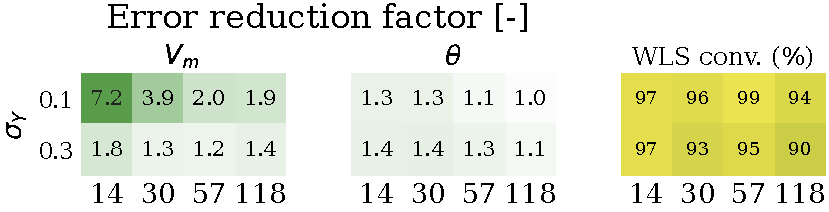
\includegraphics[width=\linewidth]{figures/se/unknown_perturbation.pdf}
    \caption{Robustness to inaccurate admittance parameters, evaluated across increasing admittance-noise levels $\sigma_Y$ (rows). The estimators are given only the base admittance matrix, before perturbation. The first two panels show the error ratio of \genco relative to the WLS baseline (ratio of median mean absolute errors) per state variable; values above $1$ (green) indicate that \genco is more accurate. The last panel depicts the convergence rate of the WLS solver; \genco always returns an estimate. Columns are the IEEE 14-, 30-, 57-, and 118-bus grids.} \label{fig:perturbation}
\end{figure}


By only adding an auxiliary decoder to the architecture discussed in \cref{sec:model}, \genco can simultaneously estimate bus states and grid parameters. We demonstrate this approach by perturbing the branch resistance/reactance ($R$, $X$) parameters with multiplicative uniform noise on $[1-\sigma', 1+\sigma']$ (half-width $\sigma'_R = \sigma'_X = 0.2$%, corresponding to an expected absolute relative deviation of $\sigma'/2 = 0.1$
) prior to inference. \genco successfully denoises the input parameters, achieving a $30$--$50\%$ reduction in noise magnitude across all tested IEEE grids. \\ %: mean relative errors on the predicted branch admittances drop consistently to a range of $0.05$--$0.07$.\\






\begin{boxH}
\paragraph{Takeaways.}
\begin{itemize}
\item SE is a task where \genco can surpass classical estimators under challenging measurement conditions. It is strongest exactly where WLS is limited by its reliance on an accurate grid model and sufficient observability:
\begin{itemize}
\item It achieves \textbf{better estimates than WLS under sparse and corrupted measurements}, although scaling this advantage to larger grids remains future work.
\item It \textbf{always returns an estimate}, maintaining good accuracy in scenarios where WLS fails to converge.
\item By treating the grid model as a soft prior rather than a hard constraint, it remains \textbf{robust to inaccurate grid parameters}.
\end{itemize}
\item The same architecture naturally extends to joint state and parameter estimation, recovering system states while denoising branch parameters.
\end{itemize}
\end{boxH}